% Options for packages loaded elsewhere
\PassOptionsToPackage{unicode}{hyperref}
\PassOptionsToPackage{hyphens}{url}
%
\documentclass[
]{book}
\usepackage{amsmath,amssymb}
\usepackage{iftex}
\ifPDFTeX
  \usepackage[T1]{fontenc}
  \usepackage[utf8]{inputenc}
  \usepackage{textcomp} % provide euro and other symbols
\else % if luatex or xetex
  \usepackage{unicode-math} % this also loads fontspec
  \defaultfontfeatures{Scale=MatchLowercase}
  \defaultfontfeatures[\rmfamily]{Ligatures=TeX,Scale=1}
\fi
\usepackage{lmodern}
\ifPDFTeX\else
  % xetex/luatex font selection
\fi
% Use upquote if available, for straight quotes in verbatim environments
\IfFileExists{upquote.sty}{\usepackage{upquote}}{}
\IfFileExists{microtype.sty}{% use microtype if available
  \usepackage[]{microtype}
  \UseMicrotypeSet[protrusion]{basicmath} % disable protrusion for tt fonts
}{}
\makeatletter
\@ifundefined{KOMAClassName}{% if non-KOMA class
  \IfFileExists{parskip.sty}{%
    \usepackage{parskip}
  }{% else
    \setlength{\parindent}{0pt}
    \setlength{\parskip}{6pt plus 2pt minus 1pt}}
}{% if KOMA class
  \KOMAoptions{parskip=half}}
\makeatother
\usepackage{xcolor}
\usepackage{color}
\usepackage{fancyvrb}
\newcommand{\VerbBar}{|}
\newcommand{\VERB}{\Verb[commandchars=\\\{\}]}
\DefineVerbatimEnvironment{Highlighting}{Verbatim}{commandchars=\\\{\}}
% Add ',fontsize=\small' for more characters per line
\usepackage{framed}
\definecolor{shadecolor}{RGB}{248,248,248}
\newenvironment{Shaded}{\begin{snugshade}}{\end{snugshade}}
\newcommand{\AlertTok}[1]{\textcolor[rgb]{0.94,0.16,0.16}{#1}}
\newcommand{\AnnotationTok}[1]{\textcolor[rgb]{0.56,0.35,0.01}{\textbf{\textit{#1}}}}
\newcommand{\AttributeTok}[1]{\textcolor[rgb]{0.13,0.29,0.53}{#1}}
\newcommand{\BaseNTok}[1]{\textcolor[rgb]{0.00,0.00,0.81}{#1}}
\newcommand{\BuiltInTok}[1]{#1}
\newcommand{\CharTok}[1]{\textcolor[rgb]{0.31,0.60,0.02}{#1}}
\newcommand{\CommentTok}[1]{\textcolor[rgb]{0.56,0.35,0.01}{\textit{#1}}}
\newcommand{\CommentVarTok}[1]{\textcolor[rgb]{0.56,0.35,0.01}{\textbf{\textit{#1}}}}
\newcommand{\ConstantTok}[1]{\textcolor[rgb]{0.56,0.35,0.01}{#1}}
\newcommand{\ControlFlowTok}[1]{\textcolor[rgb]{0.13,0.29,0.53}{\textbf{#1}}}
\newcommand{\DataTypeTok}[1]{\textcolor[rgb]{0.13,0.29,0.53}{#1}}
\newcommand{\DecValTok}[1]{\textcolor[rgb]{0.00,0.00,0.81}{#1}}
\newcommand{\DocumentationTok}[1]{\textcolor[rgb]{0.56,0.35,0.01}{\textbf{\textit{#1}}}}
\newcommand{\ErrorTok}[1]{\textcolor[rgb]{0.64,0.00,0.00}{\textbf{#1}}}
\newcommand{\ExtensionTok}[1]{#1}
\newcommand{\FloatTok}[1]{\textcolor[rgb]{0.00,0.00,0.81}{#1}}
\newcommand{\FunctionTok}[1]{\textcolor[rgb]{0.13,0.29,0.53}{\textbf{#1}}}
\newcommand{\ImportTok}[1]{#1}
\newcommand{\InformationTok}[1]{\textcolor[rgb]{0.56,0.35,0.01}{\textbf{\textit{#1}}}}
\newcommand{\KeywordTok}[1]{\textcolor[rgb]{0.13,0.29,0.53}{\textbf{#1}}}
\newcommand{\NormalTok}[1]{#1}
\newcommand{\OperatorTok}[1]{\textcolor[rgb]{0.81,0.36,0.00}{\textbf{#1}}}
\newcommand{\OtherTok}[1]{\textcolor[rgb]{0.56,0.35,0.01}{#1}}
\newcommand{\PreprocessorTok}[1]{\textcolor[rgb]{0.56,0.35,0.01}{\textit{#1}}}
\newcommand{\RegionMarkerTok}[1]{#1}
\newcommand{\SpecialCharTok}[1]{\textcolor[rgb]{0.81,0.36,0.00}{\textbf{#1}}}
\newcommand{\SpecialStringTok}[1]{\textcolor[rgb]{0.31,0.60,0.02}{#1}}
\newcommand{\StringTok}[1]{\textcolor[rgb]{0.31,0.60,0.02}{#1}}
\newcommand{\VariableTok}[1]{\textcolor[rgb]{0.00,0.00,0.00}{#1}}
\newcommand{\VerbatimStringTok}[1]{\textcolor[rgb]{0.31,0.60,0.02}{#1}}
\newcommand{\WarningTok}[1]{\textcolor[rgb]{0.56,0.35,0.01}{\textbf{\textit{#1}}}}
\usepackage{longtable,booktabs,array}
\usepackage{calc} % for calculating minipage widths
% Correct order of tables after \paragraph or \subparagraph
\usepackage{etoolbox}
\makeatletter
\patchcmd\longtable{\par}{\if@noskipsec\mbox{}\fi\par}{}{}
\makeatother
% Allow footnotes in longtable head/foot
\IfFileExists{footnotehyper.sty}{\usepackage{footnotehyper}}{\usepackage{footnote}}
\makesavenoteenv{longtable}
\usepackage{graphicx}
\makeatletter
\def\maxwidth{\ifdim\Gin@nat@width>\linewidth\linewidth\else\Gin@nat@width\fi}
\def\maxheight{\ifdim\Gin@nat@height>\textheight\textheight\else\Gin@nat@height\fi}
\makeatother
% Scale images if necessary, so that they will not overflow the page
% margins by default, and it is still possible to overwrite the defaults
% using explicit options in \includegraphics[width, height, ...]{}
\setkeys{Gin}{width=\maxwidth,height=\maxheight,keepaspectratio}
% Set default figure placement to htbp
\makeatletter
\def\fps@figure{htbp}
\makeatother
\setlength{\emergencystretch}{3em} % prevent overfull lines
\providecommand{\tightlist}{%
  \setlength{\itemsep}{0pt}\setlength{\parskip}{0pt}}
\setcounter{secnumdepth}{5}
\usepackage{booktabs}
\usepackage{amsthm}
\makeatletter
\def\thm@space@setup{%
  \thm@preskip=8pt plus 2pt minus 4pt
  \thm@postskip=\thm@preskip
}
\makeatother
\usepackage{booktabs}
\usepackage{longtable}
\usepackage{array}
\usepackage{multirow}
\usepackage{wrapfig}
\usepackage{float}
\usepackage{colortbl}
\usepackage{pdflscape}
\usepackage{tabu}
\usepackage{threeparttable}
\usepackage{threeparttablex}
\usepackage[normalem]{ulem}
\usepackage{makecell}
\usepackage{xcolor}
\ifLuaTeX
  \usepackage{selnolig}  % disable illegal ligatures
\fi
\usepackage[]{natbib}
\bibliographystyle{apalike}
\usepackage{bookmark}
\IfFileExists{xurl.sty}{\usepackage{xurl}}{} % add URL line breaks if available
\urlstyle{same}
\hypersetup{
  pdftitle={EUR/USD},
  pdfauthor={Harvey Bastidas, Andrés Caicedo, Alexander Alvarado},
  hidelinks,
  pdfcreator={LaTeX via pandoc}}

\title{EUR/USD}
\author{Harvey Bastidas, Andrés Caicedo, Alexander Alvarado}
\date{2024-11-11}

\begin{document}
\maketitle

{
\setcounter{tocdepth}{1}
\tableofcontents
}
\chapter{Justificación de elección del Dataset}\label{justificaciuxf3n-de-elecciuxf3n-del-dataset}

\textbf{Integrantes}:\\
Harvey Bastidas, Alexander Alvarado y Andrés Caicedo\\
\textbf{Materia}:\\
Análisis de series de tiempo\\
\textbf{Profesora}:\\
Isabel Cristina García

\begin{center}\rule{0.5\linewidth}{0.5pt}\end{center}

\section{Información del Dataset}\label{informaciuxf3n-del-dataset}

El dataset seleccionado para este análisis es el siguiente: \href{https://www.kaggle.com/datasets/chandrimad31/eurusd-forex-trading-data-20032021}{EUR/USD Forex Trading Data (2003-2021)}, el cual fue extraído de \href{https://forex.tradingcharts.com/}{Forex Trading Charts}, propiedad de Barchart Solutions, una empresa especializada en servicios financieros en los Estados Unidos. Barchart Solutions cuenta con reconocidos clientes como el Banco Goldman Sachs y el Bank of Canada, lo que nos lleva a concluir que los datos ofrecidos son confiables y precisos para realizar análisis financieros.

La empresa matriz, \textbf{Barchart Solutions}, tiene su sede en:

\textbf{222 S. Riverside Plaza, Suite 810,\\
Chicago, IL 60606, Estados Unidos}

El dataset presenta las tasas de cambio del par de divisas EUR/USD desde el \textbf{5 de mayo de 2003} hasta el \textbf{16 de octubre de 2021}, con una periodicidad de \textbf{4 horas}. Este conjunto de datos incluye las siguientes 6 columnas:

\begin{itemize}
\tightlist
\item
  \textbf{Open}: Precio de apertura para el periodo.
\item
  \textbf{High}: Precio máximo durante el periodo.
\item
  \textbf{Low}: Precio mínimo durante el periodo.
\item
  \textbf{Close}: Precio de cierre para el periodo.
\item
  \textbf{Volume}: Volumen de transacciones reportado.
\end{itemize}

Es importante resaltar que los datos no contienen valores nulos ni perdidos para los días de semana, aunque no se registran valores durante los fines de semana, lo que es normal en los mercados de Forex.

El análisis se centrará en la columna \textbf{Close}, que representa el precio de cierre, dado que es la variable más relevante para el pronóstico de tendencias.

\section{Justificación de la Elección del Dataset}\label{justificaciuxf3n-de-la-elecciuxf3n-del-dataset}

La elección de este dataset se fundamenta en la importancia de analizar la tasa de cambio EUR/USD, uno de los pares de divisas más negociados en el mercado Forex. La predicción de la tendencia de la tasa de cambio es crucial para varias estrategias financieras, como el balanceo de portafolios de inversión. En este contexto, se pueden usar tanto la \textbf{Teoría Moderna de Portafolios (MPT)} como la \textbf{Teoría de Portafolios Post-Moderna (PMPT)}, que son ampliamente utilizadas en la optimización de la distribución de activos. Ambas teorías se benefician de predicciones precisas de la tendencia de los activos subyacentes, como es el caso de las divisas.

Además, este dataset ofrece una excelente relación señal-ruido, lo que mejora la predictibilidad de los modelos basados en series de tiempo. Utilizamos el \textbf{coeficiente de variación (CV)} como criterio para seleccionar este dataset, debido a que es una métrica robusta para medir la variabilidad en relación con la media. Un CV bajo indica que la variabilidad en los datos es relativamente baja, lo que es favorable para la predicción de tendencias.

El \textbf{coeficiente de variación} calculado para la columna ``Close'' de este dataset es de aproximadamente \textbf{9.5\%}, lo que lo convierte en el más bajo entre los datasets que evaluamos. Esto lo hace ideal para el pronóstico, ya que un CV bajo sugiere que la señal en los datos es fuerte en comparación con el ruido.

\subsection{Relación con el Signal-to-Noise Ratio (SNR)}\label{relaciuxf3n-con-el-signal-to-noise-ratio-snr}

El \textbf{coeficiente de variación (CV)} está inversamente relacionado con el \textbf{Signal-to-Noise Ratio (SNR)}, una métrica comúnmente utilizada en el procesamiento de señales. El SNR mide la proporción de la potencia de la señal con respecto a la del ruido, lo que ayuda a evaluar la calidad de los datos.

El SNR para este dataset se calcula como el cuadrado del inverso del CV. Para el EUR/USD, con un CV de \textbf{0.09}, el SNR es aproximadamente:

\[
SNR = \left(\frac{1}{0.09}\right)^2 \approx 123
\]

Este valor indica que la señal es mucho más fuerte que el ruido en este dataset. En contraste, otro dataset que probamos, con un CV de \textbf{20\%}, tenía un SNR mucho menor, alrededor de \textbf{25}. La diferencia muestra que el dataset de EUR/USD tiene una mayor preponderancia de señal sobre el ruido, lo que permite una mejor predictibilidad en los modelos de pronóstico.

Dado que sabemos que el \textbf{SNR} es aprox \textbf{123}, esto significa que el ruido es aprox 1/123 = \textbf{0.008} que nos da una idea del máximo error absoluto (\textbf{MAE}) en los datos Normalizados en el pronósitco del siguiente periodo que podemos obtener, ya que errores por debajo de este valor probablemente incluirían la predicción del ruido y podrían ser indicador de overfitting en el modelo predictivo usado.

\section{Importancia de Analizar este Dataset}\label{importancia-de-analizar-este-dataset}

La capacidad de predecir con precisión la tasa de cambio EUR/USD tiene múltiples aplicaciones en el sector financiero. En primer lugar, es fundamental para el \textbf{trading de divisas (Forex)}, donde una mejor predicción de las tendencias puede resultar en decisiones de inversión más acertadas. Además, es esencial para la gestión de portafolios financieros, ya que permite el uso de herramientas como la \textbf{Teoría Moderna de Portafolios (MPT)}, donde la diversificación se realiza teniendo en cuenta tanto la tendencia como la variabilidad de los activos.

Por lo tanto, este dataset fue seleccionado debido a su alta calidad y baja variabilidad, lo que lo hace ideal para el análisis predictivo en el mercado de Forex, así como en la gestión de portafolios. El alto \textbf{SNR} nos da confianza en que las predicciones basadas en este dataset serán precisas y útiles en un entorno real, al mismo tiempo que nos alerta sobre los límites predictivos en función del ruido presente en los datos.

\chapter{Estructura de los datos}\label{intro}

Con el propósito de observar las tendencias y cambios estructurales en la serie, se realizan pruebas estadísticas para conocer la estructura subyacente de la serie.

\section{Cálculo de Medias Móviles Simples:}\label{cuxe1lculo-de-medias-muxf3viles-simples}

El cálculo de medias móviles es una técnica común en el análisis de series de tiempo utilizada para suavizar las fluctuaciones a corto plazo y destacar las tendencias subyacentes en los datos. En este análisis, se implementan medias móviles de corto y largo plazo para identificar patrones de comportamiento y ayudar en la toma de decisiones basadas en tendencias más claras.

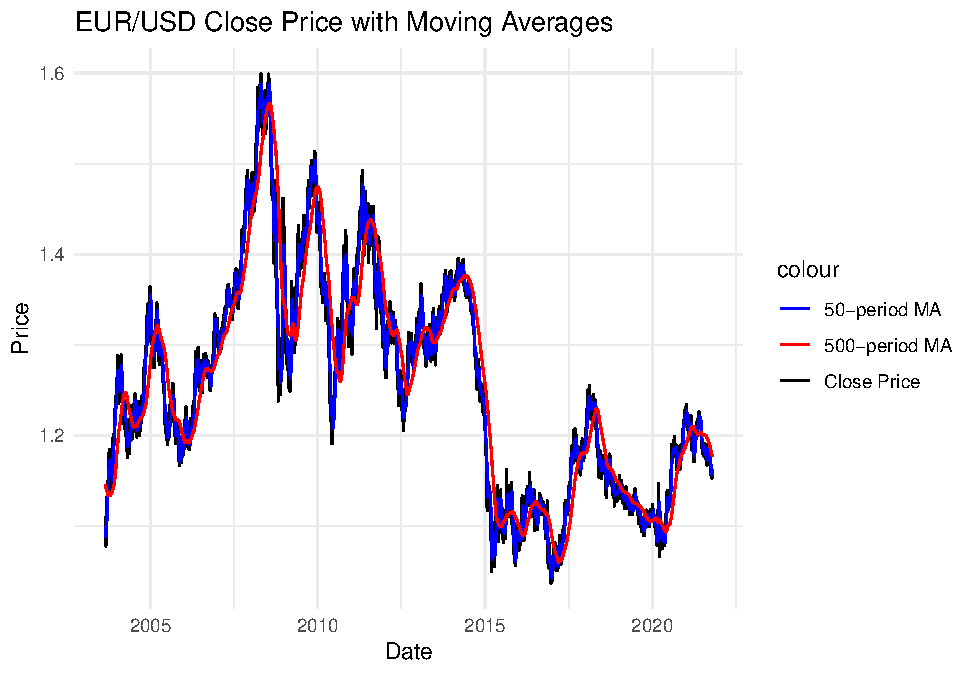
\includegraphics{bookdown_time_series_files/figure-latex/unnamed-chunk-3-1.pdf}

\begin{itemize}
\item
  \textbf{Media móvil de 50 periodos (MA corta)}:

  \begin{itemize}
  \item
    Sigue de cerca las fluctuaciones del precio de cierre, respondiendo rápidamente a los cambios de tendencia.
  \item
    Captura las tendencias a \textbf{corto plazo}, pero también refleja mucha volatilidad.
  \end{itemize}
\item
  \textbf{Media móvil de 500 periodos (MA larga)}:

  \begin{itemize}
  \item
    Se mueve de forma más suave, reaccionando más lentamente a los cambios de precios.
  \item
    Indica la \textbf{tendencia a largo plazo}, proporcionando una visión más estable del comportamiento del mercado.
  \end{itemize}
\end{itemize}

\section{Análisis de Rezagos}\label{anuxe1lisis-de-rezagos}

Cómo se comporta la serie de tiempo con respecto a sus valores pasados, introduciendo rezagos.

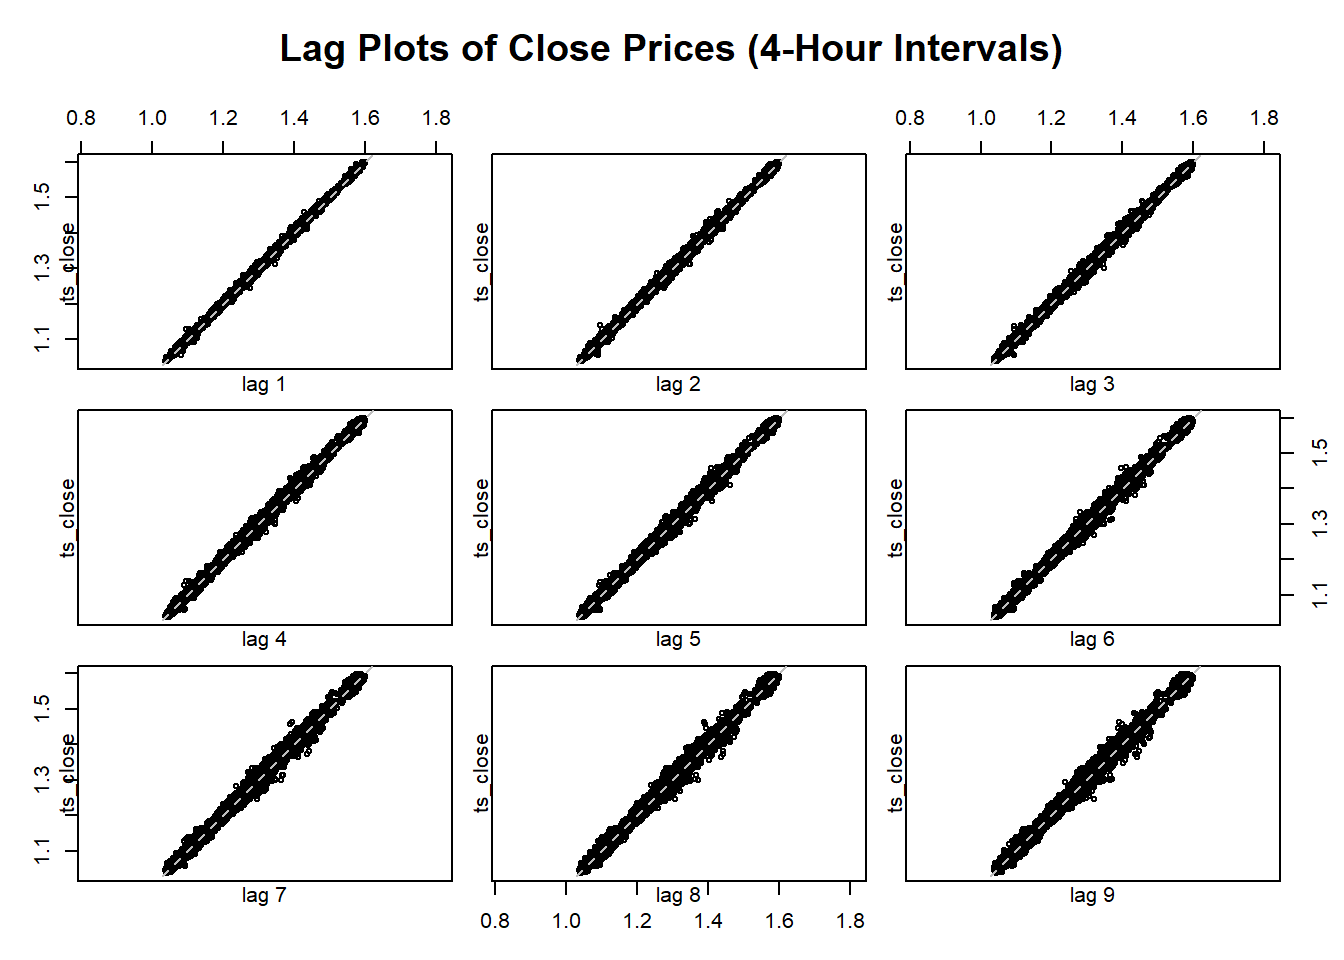
\includegraphics{bookdown_time_series_files/figure-latex/unnamed-chunk-5-1.pdf}

En cada uno de los gráficos, los puntos siguen una línea casi perfectamente recta, sugiriendo una \textbf{alta autocorrelación} entre los valores de la serie con sus rezagos cercanos.

La pendiente positiva indica que cuando el valor anterior era alto, el valor actual también tiende a ser alto, y lo mismo sucede para valores bajos. Esto sugiere que \textbf{la serie es muy persistente}, es decir, los precios tienden a seguir una dirección similar en el corto plazo.

Dado que no hay patrones dispersos o sin forma definida, se puede inferir que la serie no tiene cambios abruptos o comportamiento caótico entre los puntos cercanos. Esto podría indicar que \textbf{no hay mucha volatilidad} en los intervalos de 4 horas.

\section{Análisis de Estacionalidad}\label{anuxe1lisis-de-estacionalidad}

Para detectar si existe estacionalidad (patrones repetitivos), utilizaremos \textbf{decomposición} o \textbf{test de estacionalidad}.

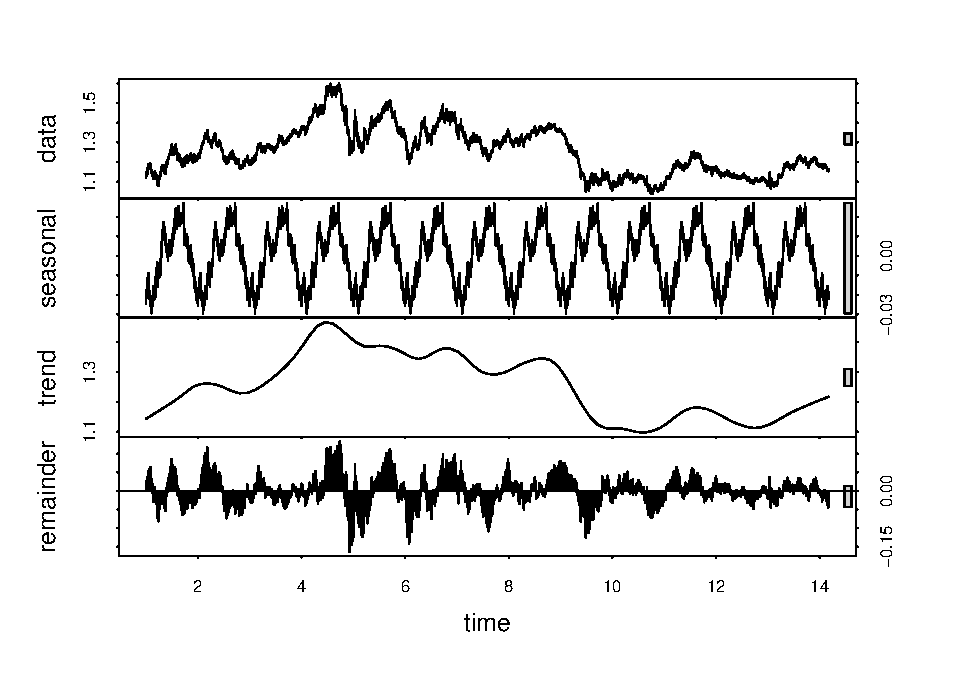
\includegraphics{bookdown_time_series_files/figure-latex/unnamed-chunk-6-1.pdf}

En la gráfica de \textbf{descomposición de series de tiempo} se visualizan los \textbf{componentes de la serie}: datos originales, estacionalidad, tendencia y residuales (remainder):

1. \textbf{Datos Originales (data):} En la primera gráfica (data), se observan los valores de cierre a lo largo del tiempo. Vemos fluctuaciones en los precios con algunas subidas y bajadas claras, lo que indica la volatilidad normal del mercado Forex.

2. \textbf{Componente Estacional (seasonal):} El segundo gráfico muestra un \textbf{patrón repetitivo y periódico}. Este patrón sugiere que hay \textbf{ciclos regulares} en la serie. La estacionalidad se mantiene constante a lo largo del tiempo, lo que indica que ciertos movimientos en el mercado se repiten con una periodicidad fija (en este caso, podría ser diaria o semanal). Es probable que este componente estacional refleje la actividad cíclica en horarios específicos o días determinados, como mayor volatilidad durante sesiones overlap (como entre Londres y Nueva York).

3. \textbf{Componente de Tendencia (trend):} El tercer gráfico muestra una \textbf{tendencia suavizada} que sigue la dirección general del mercado. Observamos fases de \textbf{alzas y caídas}: primero hay una subida clara, luego una caída, y finalmente otra leve tendencia hacia la estabilidad.

4. \textbf{Componente de Residuos o Resto (remainder):} El último gráfico (remainder) muestra los \textbf{residuos} o la parte de los datos que no es explicada por la tendencia ni la estacionalidad. Estos residuos parecen ser \textbf{ruido blanco}, con fluctuaciones alrededor de cero, lo que indica que no hay patrones significativos adicionales no capturados por los otros componentes.

\chapter{Preprocesamiento y Visualización}\label{preprocesamiento-y-visualizaciuxf3n}

En este análisis, trabajaremos con el dataset de tipo de cambio EUR/USD de Forex proporcionado, el cual incluye datos históricos de 2003 a 2021. El objetivo es estudiar las tendencias, estacionalidad y comportamiento estructural de la serie de tiempo. Además, evaluaremos si es necesario realizar transformaciones en la serie para estabilizar la varianza y facilitar la predicción.

\section{Descomposición de la Serie de Tiempo}\label{descomposiciuxf3n-de-la-serie-de-tiempo}

En esta etapa se busca realizar la descomposición de la serie de tiempo para identificar los componentes de \textbf{tendencia}, \textbf{estacionalidad} y \textbf{residuos}.

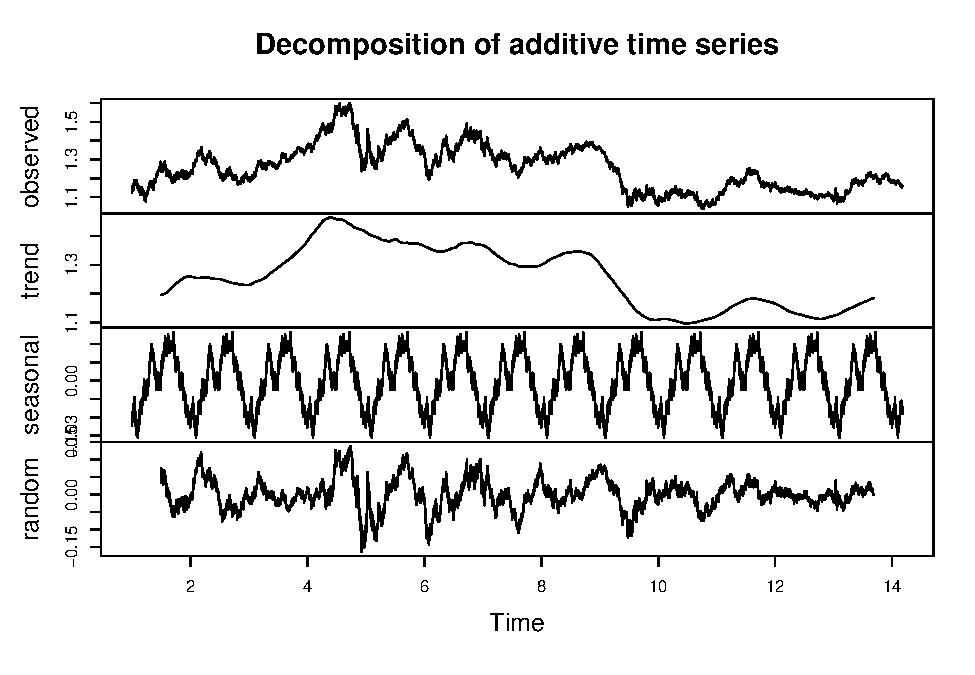
\includegraphics{bookdown_time_series_files/figure-latex/unnamed-chunk-8-1.pdf}

En la gráfica de \textbf{descomposición de series de tiempo} se visualizan los \textbf{componentes de la serie}: datos originales, estacionalidad, tendencia y residuales (remainder):

1. \textbf{Datos Originales (data):} En la primera gráfica (data), se observan los valores de cierre a lo largo del tiempo. Vemos fluctuaciones en los precios con algunas subidas y bajadas claras, lo que indica la volatilidad normal del mercado Forex.

2. \textbf{Componente Estacional (seasonal):} El segundo gráfico muestra un \textbf{patrón repetitivo y periódico}. Este patrón sugiere que hay \textbf{ciclos regulares} en la serie. La estacionalidad se mantiene constante a lo largo del tiempo, lo que indica que ciertos movimientos en el mercado se repiten con una periodicidad fija (en este caso, podría ser diaria o semanal). Es probable que este componente estacional refleje la actividad cíclica en horarios específicos o días determinados, como mayor volatilidad durante sesiones overlap (como entre Londres y Nueva York).

3. \textbf{Componente de Tendencia (trend):} El tercer gráfico muestra una \textbf{tendencia suavizada} que sigue la dirección general del mercado. Observamos fases de \textbf{alzas y caídas}: primero hay una subida clara, luego una caída, y finalmente otra leve tendencia hacia la estabilidad.

4. \textbf{Componente de Residuos o Resto (remainder):} El último gráfico (remainder) muestra los \textbf{residuos} o la parte de los datos que no es explicada por la tendencia ni la estacionalidad. Estos residuos parecen ser \textbf{ruido blanco}, con fluctuaciones alrededor de cero, lo que indica que no hay patrones significativos adicionales no capturados por los otros componentes.

\section{Prueba de Estacionariedad}\label{prueba-de-estacionariedad}

La estacionariedad es importante en el análisis de series de tiempo porque indica si las propiedades estadísticas de la serie (como la media y la varianza) se mantienen constantes a lo largo del tiempo. Una serie estacionaria es generalmente más fácil de modelar y predecir.

\begin{verbatim}
## Augmented Dickey-Fuller Test 
## alternative: stationary 
##  
## Type 1: no drift no trend 
##       lag    ADF p.value
##  [1,]   0 -0.135   0.606
##  [2,]   1 -0.133   0.606
##  [3,]   2 -0.135   0.606
##  [4,]   3 -0.131   0.607
##  [5,]   4 -0.143   0.603
##  [6,]   5 -0.146   0.603
##  [7,]   6 -0.149   0.602
##  [8,]   7 -0.147   0.602
##  [9,]   8 -0.155   0.600
## [10,]   9 -0.156   0.600
## [11,]  10 -0.158   0.599
## [12,]  11 -0.174   0.594
## [13,]  12 -0.172   0.595
## [14,]  13 -0.169   0.596
## [15,]  14 -0.166   0.597
## Type 2: with drift no trend 
##       lag   ADF p.value
##  [1,]   0 -2.20   0.248
##  [2,]   1 -2.21   0.244
##  [3,]   2 -2.23   0.238
##  [4,]   3 -2.19   0.253
##  [5,]   4 -2.20   0.250
##  [6,]   5 -2.20   0.248
##  [7,]   6 -2.21   0.244
##  [8,]   7 -2.20   0.248
##  [9,]   8 -2.19   0.254
## [10,]   9 -2.18   0.257
## [11,]  10 -2.18   0.255
## [12,]  11 -2.18   0.257
## [13,]  12 -2.18   0.257
## [14,]  13 -2.16   0.263
## [15,]  14 -2.17   0.258
## Type 3: with drift and trend 
##       lag   ADF p.value
##  [1,]   0 -2.91   0.192
##  [2,]   1 -2.93   0.186
##  [3,]   2 -2.94   0.180
##  [4,]   3 -2.90   0.196
##  [5,]   4 -2.90   0.197
##  [6,]   5 -2.90   0.196
##  [7,]   6 -2.91   0.193
##  [8,]   7 -2.90   0.197
##  [9,]   8 -2.88   0.207
## [10,]   9 -2.87   0.210
## [11,]  10 -2.87   0.209
## [12,]  11 -2.85   0.219
## [13,]  12 -2.85   0.218
## [14,]  13 -2.84   0.223
## [15,]  14 -2.85   0.216
## ---- 
## Note: in fact, p.value = 0.01 means p.value <= 0.01
\end{verbatim}

\begin{verbatim}
## $type1
##       lag        ADF   p.value
##  [1,]   0 -0.1349353 0.6056581
##  [2,]   1 -0.1332845 0.6061322
##  [3,]   2 -0.1350012 0.6056392
##  [4,]   3 -0.1311022 0.6067589
##  [5,]   4 -0.1432485 0.6032707
##  [6,]   5 -0.1455745 0.6026027
##  [7,]   6 -0.1491280 0.6015823
##  [8,]   7 -0.1466525 0.6022932
##  [9,]   8 -0.1553530 0.5997946
## [10,]   9 -0.1558747 0.5996447
## [11,]  10 -0.1575228 0.5991714
## [12,]  11 -0.1743717 0.5943327
## [13,]  12 -0.1723248 0.5949206
## [14,]  13 -0.1686293 0.5959819
## [15,]  14 -0.1662663 0.5966605
## 
## $type2
##       lag       ADF   p.value
##  [1,]   0 -2.199690 0.2481241
##  [2,]   1 -2.210308 0.2438767
##  [3,]   2 -2.225752 0.2376991
##  [4,]   3 -2.186315 0.2534741
##  [5,]   4 -2.196090 0.2495641
##  [6,]   5 -2.199991 0.2480038
##  [7,]   6 -2.210932 0.2436273
##  [8,]   7 -2.199519 0.2481923
##  [9,]   8 -2.185380 0.2538481
## [10,]   9 -2.178336 0.2566657
## [11,]  10 -2.183564 0.2545744
## [12,]  11 -2.178602 0.2565592
## [13,]  12 -2.178490 0.2566041
## [14,]  13 -2.163515 0.2625942
## [15,]  14 -2.174827 0.2580694
## 
## $type3
##       lag       ADF   p.value
##  [1,]   0 -2.911720 0.1919072
##  [2,]   1 -2.925278 0.1861988
##  [3,]   2 -2.940306 0.1798712
##  [4,]   3 -2.902268 0.1958871
##  [5,]   4 -2.899542 0.1970351
##  [6,]   5 -2.901407 0.1962497
##  [7,]   6 -2.909540 0.1928254
##  [8,]   7 -2.900196 0.1967594
##  [9,]   8 -2.875536 0.2071427
## [10,]   9 -2.867569 0.2104971
## [11,]  10 -2.871608 0.2087965
## [12,]  11 -2.848029 0.2187245
## [13,]  12 -2.850350 0.2177475
## [14,]  13 -2.838511 0.2227323
## [15,]  14 -2.853430 0.2164506
\end{verbatim}

La interpretación es la siguiente:

\begin{itemize}
\item
  \textbf{Hipótesis nula (H0)}: La serie no es estacionaria (tiene una raíz unitaria).
\item
  \textbf{Hipótesis alternativa (H1)}: La serie es estacionaria.
\end{itemize}

En todas las configuraciones (sin tendencia ni drift, con drift, y con drift y tendencia), los p-valores son mayores a 0.05. Esto implica que, bajo ninguna de estas configuraciones, la serie es estacionaria en su forma actual.

\section{Diferenciación para Estacionariedad}\label{diferenciaciuxf3n-para-estacionariedad}

Como la serie no es estacionaria, el siguiente paso es aplicar una diferenciación para intentar volverla estacionaria. La diferenciación ayuda a eliminar tendencias y hacer que las propiedades estadísticas de la serie se mantengan constantes a lo largo del tiempo.

Aplicaremos una diferenciación de primer orden y realizaremos nuevamente la prueba ADF para verificar si la serie se ha vuelto estacionaria.

Para este análisis, utilizaremos la columna de cierre (\texttt{Close}) del dataset como nuestra serie de tiempo principal. Convertiremos los datos a formato de serie temporal.

Aplicaremos una primera diferenciación.

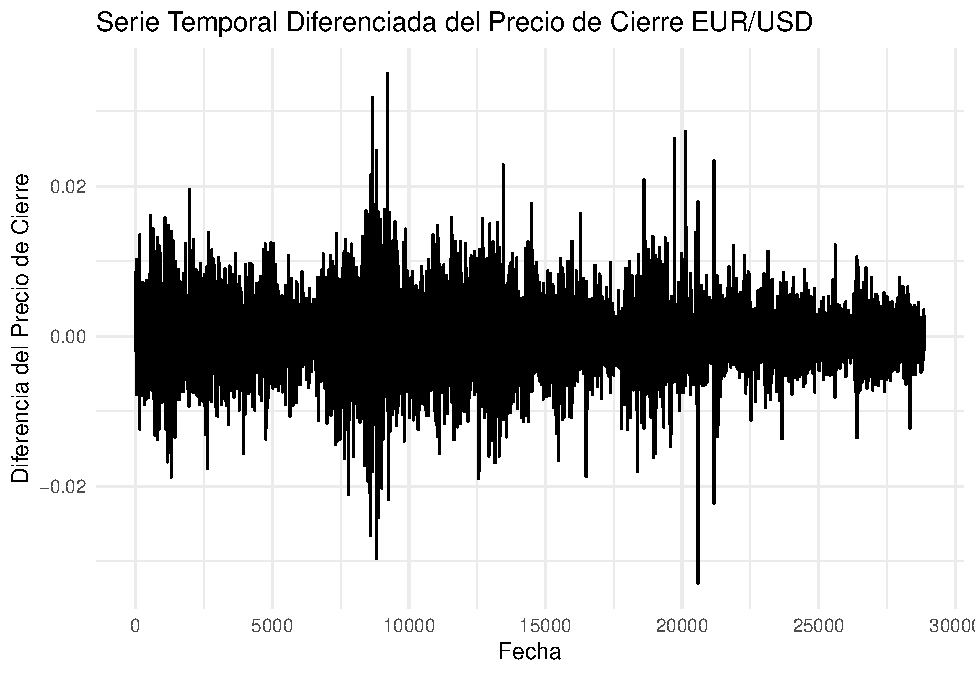
\includegraphics{bookdown_time_series_files/figure-latex/differencing-1.pdf}

Después de la primera diferenciación, se puede obtener que por cada tick quedó el valor del return (x-x\_ant) ue es el resultado de la aplicación de la dirferenciaciónd e primer orden. Como se aprecia, la serie ya no tiene una tendencia sino que presenta un comportamiento estacionario, sinembargo, esta serie de tiempo parece ser menos predecible que la serie de tiempo antes de la diferenciación, ya que evidentemente tiene mayor desviación estándar y por tanto un mayor Coeficiente de Variación y un menor SNR.

\section{Verificación de Estacionariedad en la Serie Diferenciada}\label{verificaciuxf3n-de-estacionariedad-en-la-serie-diferenciada}

Aplicamos nuevamente la prueba Dickey-Fuller a la serie diferenciada para verificar si ahora es estacionaria.

\begin{verbatim}
## Augmented Dickey-Fuller Test 
## alternative: stationary 
##  
## Type 1: no drift no trend 
##       lag    ADF p.value
##  [1,]   0 -169.3    0.01
##  [2,]   1 -119.0    0.01
##  [3,]   2  -99.3    0.01
##  [4,]   3  -84.8    0.01
##  [5,]   4  -75.7    0.01
##  [6,]   5  -68.7    0.01
##  [7,]   6  -64.1    0.01
##  [8,]   7  -60.1    0.01
##  [9,]   8  -56.8    0.01
## [10,]   9  -53.7    0.01
## [11,]  10  -50.9    0.01
## [12,]  11  -48.8    0.01
## [13,]  12  -47.3    0.01
## [14,]  13  -45.4    0.01
## [15,]  14  -43.7    0.01
## Type 2: with drift no trend 
##       lag    ADF p.value
##  [1,]   0 -169.3    0.01
##  [2,]   1 -119.0    0.01
##  [3,]   2  -99.3    0.01
##  [4,]   3  -84.8    0.01
##  [5,]   4  -75.7    0.01
##  [6,]   5  -68.7    0.01
##  [7,]   6  -64.1    0.01
##  [8,]   7  -60.1    0.01
##  [9,]   8  -56.8    0.01
## [10,]   9  -53.7    0.01
## [11,]  10  -50.9    0.01
## [12,]  11  -48.8    0.01
## [13,]  12  -47.3    0.01
## [14,]  13  -45.4    0.01
## [15,]  14  -43.7    0.01
## Type 3: with drift and trend 
##       lag    ADF p.value
##  [1,]   0 -169.3    0.01
##  [2,]   1 -119.0    0.01
##  [3,]   2  -99.3    0.01
##  [4,]   3  -84.9    0.01
##  [5,]   4  -75.7    0.01
##  [6,]   5  -68.7    0.01
##  [7,]   6  -64.1    0.01
##  [8,]   7  -60.1    0.01
##  [9,]   8  -56.8    0.01
## [10,]   9  -53.7    0.01
## [11,]  10  -50.9    0.01
## [12,]  11  -48.8    0.01
## [13,]  12  -47.3    0.01
## [14,]  13  -45.4    0.01
## [15,]  14  -43.7    0.01
## ---- 
## Note: in fact, p.value = 0.01 means p.value <= 0.01
\end{verbatim}

\begin{verbatim}
## $type1
##       lag        ADF p.value
##  [1,]   0 -169.27722    0.01
##  [2,]   1 -119.03874    0.01
##  [3,]   2  -99.30334    0.01
##  [4,]   3  -84.84969    0.01
##  [5,]   4  -75.69590    0.01
##  [6,]   5  -68.70703    0.01
##  [7,]   6  -64.07591    0.01
##  [8,]   7  -60.05652    0.01
##  [9,]   8  -56.77621    0.01
## [10,]   9  -53.68723    0.01
## [11,]  10  -50.91061    0.01
## [12,]  11  -48.81278    0.01
## [13,]  12  -47.29027    0.01
## [14,]  13  -45.38630    0.01
## [15,]  14  -43.68676    0.01
## 
## $type2
##       lag        ADF p.value
##  [1,]   0 -169.27433    0.01
##  [2,]   1 -119.03671    0.01
##  [3,]   2  -99.30166    0.01
##  [4,]   3  -84.84825    0.01
##  [5,]   4  -75.69462    0.01
##  [6,]   5  -68.70587    0.01
##  [7,]   6  -64.07484    0.01
##  [8,]   7  -60.05550    0.01
##  [9,]   8  -56.77525    0.01
## [10,]   9  -53.68632    0.01
## [11,]  10  -50.90973    0.01
## [12,]  11  -48.81194    0.01
## [13,]  12  -47.28946    0.01
## [14,]  13  -45.38553    0.01
## [15,]  14  -43.68601    0.01
## 
## $type3
##       lag        ADF p.value
##  [1,]   0 -169.27489    0.01
##  [2,]   1 -119.03832    0.01
##  [3,]   2  -99.30402    0.01
##  [4,]   3  -84.85094    0.01
##  [5,]   4  -75.69772    0.01
##  [6,]   5  -68.70929    0.01
##  [7,]   6  -64.07866    0.01
##  [8,]   7  -60.05942    0.01
##  [9,]   8  -56.77944    0.01
## [10,]   9  -53.69075    0.01
## [11,]  10  -50.91391    0.01
## [12,]  11  -48.81642    0.01
## [13,]  12  -47.29426    0.01
## [14,]  13  -45.39063    0.01
## [15,]  14  -43.69120    0.01
\end{verbatim}

\section{Justificación de la Transformación}\label{justificaciuxf3n-de-la-transformaciuxf3n}

Dado que la serie original no era estacionaria, fue necesario aplicar una diferenciación de primer orden para hacerla estacionaria. Esta transformación es importante para poder aplicar modelos de series de tiempo que asumen estacionariedad y para obtener mejores resultados en el análisis de patrones y predicciones.

\section{Análisis de Autocorrelación}\label{anuxe1lisis-de-autocorrelaciuxf3n}

Graficaremos las funciones de autocorrelación (ACF) y autocorrelación parcial (PACF) para observar la dependencia temporal en los datos diferenciados.

\begin{Shaded}
\begin{Highlighting}[]
\CommentTok{\# Graficar ACF y PACF de la serie diferenciada}
\FunctionTok{par}\NormalTok{(}\AttributeTok{mfrow =} \FunctionTok{c}\NormalTok{(}\DecValTok{1}\NormalTok{, }\DecValTok{2}\NormalTok{))}
\FunctionTok{Acf}\NormalTok{(forex\_diff, }\AttributeTok{main =} \StringTok{"ACF de la Serie Diferenciada"}\NormalTok{)}
\FunctionTok{Pacf}\NormalTok{(forex\_diff, }\AttributeTok{main =} \StringTok{"PACF de la Serie Diferenciada"}\NormalTok{)}
\end{Highlighting}
\end{Shaded}

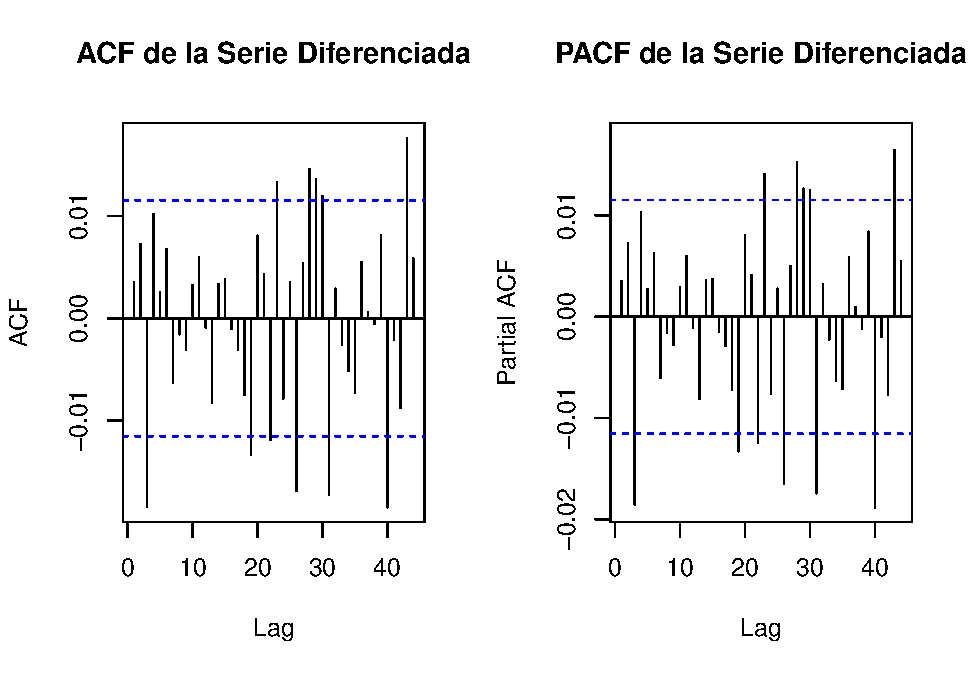
\includegraphics{bookdown_time_series_files/figure-latex/acf-pacf-1.pdf}

\begin{Shaded}
\begin{Highlighting}[]
\FunctionTok{par}\NormalTok{(}\AttributeTok{mfrow =} \FunctionTok{c}\NormalTok{(}\DecValTok{1}\NormalTok{,}\DecValTok{1}\NormalTok{))}
\end{Highlighting}
\end{Shaded}

La ACF a la izquierda muestra cómo los valores actuales de la serie diferenciada están correlacionados con sus valores en diferentes rezagos (lags). Algunos puntos de la ACF están fuera de las líneas de significancia (líneas punteadas azules), lo cual sugiere que hay correlaciones significativas en esos rezagos específicos. Este patrón puede ser indicativo de que aún existen estructuras autoregresivas o de medias móviles en la serie, incluso después de la diferenciación.

La PACF a la derecha muestra la autocorrelación de la serie diferenciada en cada rezago eliminando el efecto de los rezagos intermedios. Similar a la ACF, algunos valores están fuera de las líneas de significancia, lo que indica correlación significativa en esos rezagos específicos. Este patrón puede sugerir la presencia de efectos autoregresivos en los rezagos correspondientes.

Los picos significativos en la ACF y PACF sugieren que la serie diferenciada podría beneficiarse de un modelo ARIMA para capturar la estructura subyacente. Dependiendo de la cantidad de rezagos significativos en cada gráfico, podría ser apropiado un modelo ARIMA específico (por ejemplo, con ciertos órdenes autoregresivos y de medias móviles).

\section{Modelo ARIMA}\label{modelo-arima}

Utilizaremos \texttt{auto.arima} para identificar el mejor modelo ARIMA para los datos.

\begin{Shaded}
\begin{Highlighting}[]
\CommentTok{\# Ajuste del modelo ARIMA}
\NormalTok{forex\_arima }\OtherTok{\textless{}{-}} \FunctionTok{auto.arima}\NormalTok{(forex\_diff)}
\FunctionTok{summary}\NormalTok{(forex\_arima)}
\end{Highlighting}
\end{Shaded}

\begin{verbatim}
## Series: forex_diff 
## ARIMA(0,0,0) with zero mean 
## 
## sigma^2 = 8.978e-06:  log likelihood = 126732.8
## AIC=-253463.6   AICc=-253463.6   BIC=-253455.4
## 
## Training set error measures:
##                        ME        RMSE         MAE MPE MAPE     MASE        ACF1
## Training set 1.304966e-06 0.002996269 0.001979825 100  100 0.675058 0.003518741
\end{verbatim}

El modelo ajustado para la serie forex\_diff es un ARIMA(0,0,0) con media cero, lo que sugiere que la serie no presenta patrones autoregresivos ni de medias móviles significativos, siendo esencialmente ruido blanco. El valor de sigma\^{}2 = 8.978×10 −6 representa la varianza del error, con una alta verosimilitud (log likelihood) de 126732.8. Los criterios de información, AIC y BIC, son de -253463.6 y -253455.4, respectivamente, indicando un buen ajuste para este modelo sencillo. Las medidas de error en el conjunto de entrenamiento muestran un error medio (ME) cercano a cero (1.30e-06) y un RMSE de 0.002996, lo cual refleja una precisión razonable. La autocorrelación en el primer rezago (ACF1) es baja (0.0035), sugiriendo independencia en los residuos.

\section{Detección de Puntos de Cambio}\label{detecciuxf3n-de-puntos-de-cambio}

Usaremos la función \texttt{cpt.mean} para detectar cambios significativos en la media de la serie.

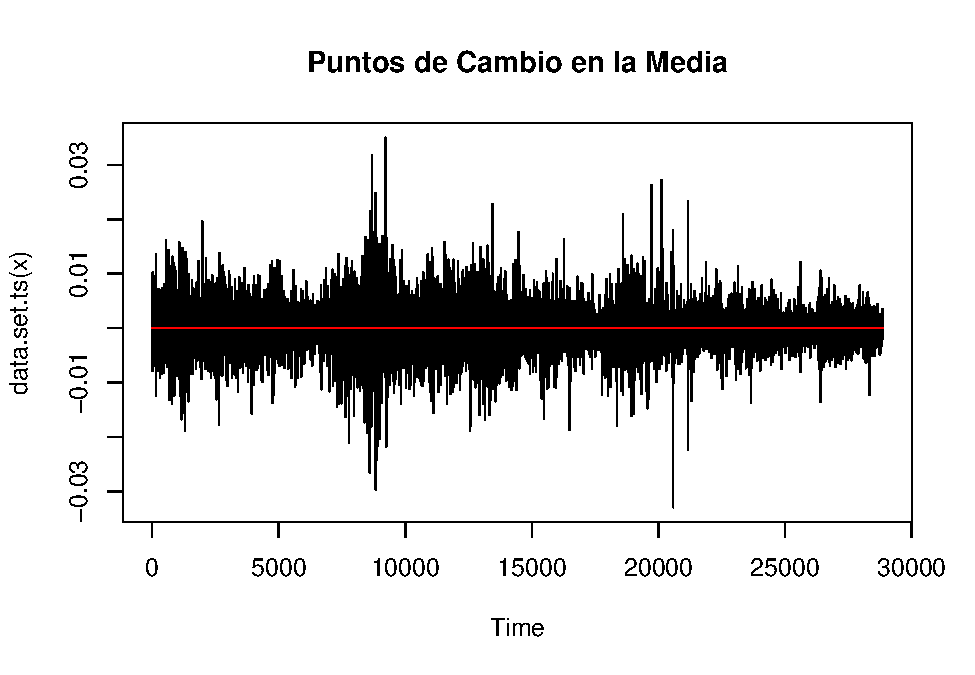
\includegraphics{bookdown_time_series_files/figure-latex/change-point-1.pdf}

No se detectaron puntos de cambio, debido a que después de la diferenciación, se convierte básicamente en ruido blanco.

\section{Media Cero de los Residuos}\label{media-cero-de-los-residuos}

Comprobamos si la media de los residuos es cero.

\begin{Shaded}
\begin{Highlighting}[]
\CommentTok{\# Prueba t en los residuos}
\NormalTok{residuals\_arima }\OtherTok{\textless{}{-}} \FunctionTok{residuals}\NormalTok{(forex\_arima)}
\NormalTok{t\_test\_residuals }\OtherTok{\textless{}{-}} \FunctionTok{t.test}\NormalTok{(residuals\_arima)}
\FunctionTok{print}\NormalTok{(t\_test\_residuals)}
\end{Highlighting}
\end{Shaded}

\begin{verbatim}
## 
##  One Sample t-test
## 
## data:  residuals_arima
## t = 0.073986, df = 28858, p-value = 0.941
## alternative hypothesis: true mean is not equal to 0
## 95 percent confidence interval:
##  -3.326619e-05  3.587612e-05
## sample estimates:
##    mean of x 
## 1.304966e-06
\end{verbatim}

La prueba t de una muestra realizada sobre los residuos (residuals\_arima) arroja un valor de 𝑡=0.073986 con 28,858 grados de libertad y un valor p de 0.941. Dado que el valor p es significativamente mayor a 0.05, no rechazamos la hipótesis nula de que la media de los residuos es igual a cero. Esto sugiere que los residuos no presentan un sesgo significativo. El intervalo de confianza del 95\% para la media de los residuos y la media estimada muy cercana a cero es consistente con un modelo bien ajustado sin tendencia sistemática en los errores.

\section{Independencia de los Residuos}\label{independencia-de-los-residuos}

Evaluamos la independencia de los residuos usando la prueba de Ljung-Box.

\begin{Shaded}
\begin{Highlighting}[]
\CommentTok{\# Prueba de independencia}
\FunctionTok{Box.test}\NormalTok{(residuals\_arima, }\AttributeTok{lag =} \DecValTok{20}\NormalTok{, }\AttributeTok{type =} \StringTok{"Ljung{-}Box"}\NormalTok{)}
\end{Highlighting}
\end{Shaded}

\begin{verbatim}
## 
##  Box-Ljung test
## 
## data:  residuals_arima
## X-squared = 30.772, df = 20, p-value = 0.05827
\end{verbatim}

Los datos cargados contienen 28,860 filas y 6 columnas de información sobre el tipo de cambio EUR/USD. La prueba de Dickey-Fuller Aumentada (ADF) realizada en tres configuraciones (sin constante ni tendencia, con constante sin tendencia, y con constante y tendencia) muestra valores ADF altamente negativos y p-valores menores o iguales a 0.01, lo que indica que la serie diferenciada es estacionaria. Además, la prueba de Box-Ljung aplicada a los residuos del modelo ARIMA arroja un valor de 30.772 con un valor p de 0.05827, lo cual sugiere que los residuos \textbf{no tienen autocorrelación significativa}, indicando independencia en los errores del modelo.

\section{Distribución de los Residuos}\label{distribuciuxf3n-de-los-residuos}

Analizaremos la normalidad de los residuos con un gráfico Q-Q.

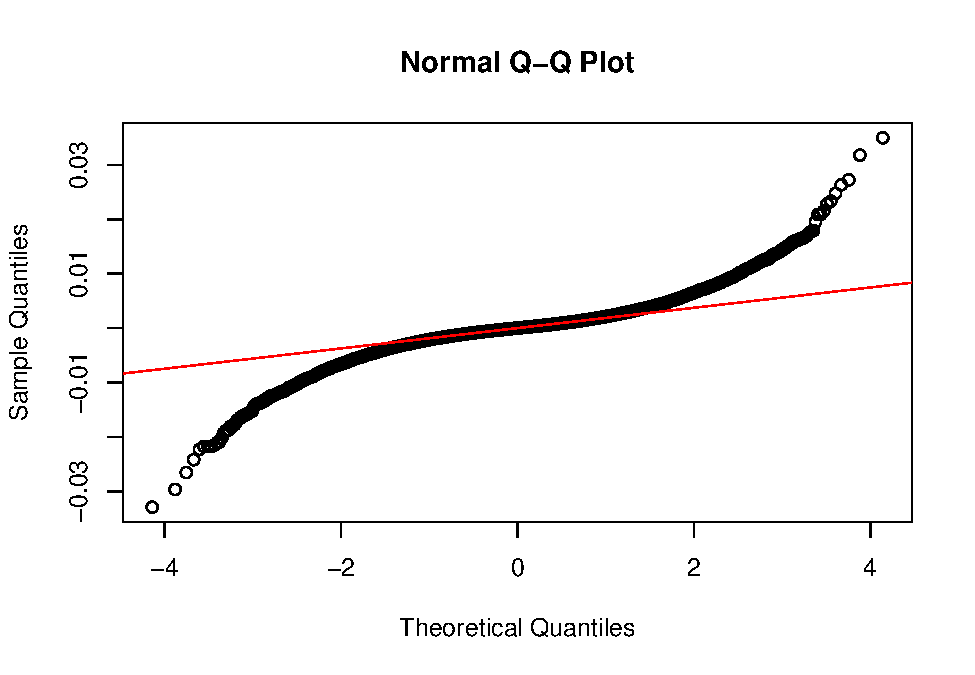
\includegraphics{bookdown_time_series_files/figure-latex/residuals-qqplot-1.pdf}

El gráfico Q-Q muestra que los residuos del modelo se alinean con la normalidad en el centro de la distribución, pero presentan desviaciones significativas en las colas. Esto sugiere que, aunque los residuos se comportan aproximadamente como una distribución normal en el centro, tienen colas más pesadas de lo esperado, lo que indica la presencia de valores extremos.

\chapter{Análisis de Series de Tiempo con el Método Holt-Winters}\label{anuxe1lisis-de-series-de-tiempo-con-el-muxe9todo-holt-winters}

Este documento realiza un análisis de series de tiempo utilizando el método de Holt-Winters aplicado exclusivamente a la columna \texttt{close} del dataset \texttt{EURUSD\_ForexTrading\_4hrs.csv}. Se utilizarán solo 6000 datos, normalizando la columna \texttt{close}, dividiendo en conjunto de entrenamiento y prueba, y calculando la métricas de error MAE en el conjunto de entrenamiento y en el conjunto de prueba.

\section{Carga de Bibliotecas y Datos}\label{carga-de-bibliotecas-y-datos}

\begin{table}
\centering
\caption{\label{tab:cargar-datos}Primeras filas del dataset EURUSD ForexTrading 4hrs Columna close}
\centering
\begin{tabular}[t]{r}
\hline
close\\
\hline
1.12274\\
\hline
1.12126\\
\hline
1.12113\\
\hline
1.12174\\
\hline
1.12712\\
\hline
1.12804\\
\hline
\end{tabular}
\end{table}

El dataset \texttt{EURUSD\_ForexTrading\_4hrs.csv} contiene datos de trading del par de divisas EUR/USD con una frecuencia de 4 horas. Solo se ha seleccionado la columna \texttt{close} con los primeros 6000 datos para este análisis.

\section{Normalización de la Columna `close'}\label{normalizaciuxf3n-de-la-columna-close}

\begin{table}
\centering
\caption{\label{tab:normalizar-close}Columna 'close' Normalizada}
\centering
\begin{tabular}[t]{r}
\hline
x\\
\hline
0.1566893\\
\hline
0.1515141\\
\hline
0.1510595\\
\hline
0.1531925\\
\hline
0.1720050\\
\hline
0.1752220\\
\hline
\end{tabular}
\end{table}

Se ha normalizado la columna \texttt{close} utilizando la técnica Min-Max, transformando los valores entre 0 y 1 para mejorar la estabilidad del modelo.

\section{Descomposición Estacional}\label{descomposiciuxf3n-estacional}

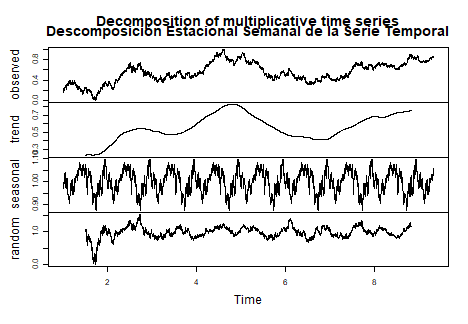
\includegraphics{bookdown_time_series_files/figure-latex/descomposicion-estacional-1.png}

Descomponemos la serie temporal en componentes de tendencia, estacionalidad y ruido para analizar los patrones internos de la serie temporal antes de aplicar el modelo.

\section{Suavizado Exponencial Simple}\label{suavizado-exponencial-simple}

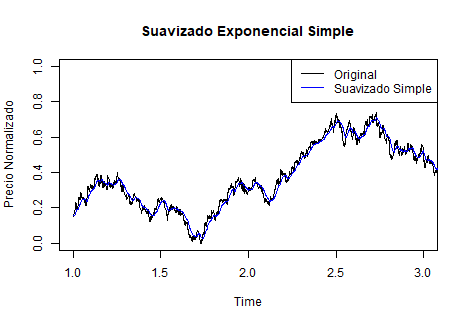
\includegraphics{bookdown_time_series_files/figure-latex/suavizado-simple-1.png}

Aplicamos el suavizado exponencial simple a la serie \texttt{close} para visualizar una versión suavizada de la serie de tiempo. Se pude observar como la señal original contiene mas ruido que la suavizada.

\section{Suavizado Exponencial Doble (Aditivo y Multiplicativo)}\label{suavizado-exponencial-doble-aditivo-y-multiplicativo}

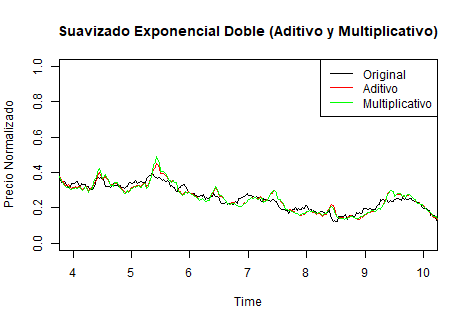
\includegraphics{bookdown_time_series_files/figure-latex/suavizado-doble-1.png}

Se puede apreciar que tanto el suavizado aditivo como el multiplicativo producen una estimación cercana a los datos originales, aunque estas señales contienen mas ruido que el suavizado simple e incluso al parecer mas que la señal original.

\section{Calculo de error}\label{calculo-de-error}

Se calcularon los errores de los modelos multiplicativo y aditivo en el dataset de training. Se usa un ajuste de 0.001 para el modelo multiplicativo, porque este requiere que todos los datos sean positivos y mayores que cero (no admite ceros), y como los datos fueron nomalizados con min-max, obligatoriamente existe al menos un valor de cero.

\begin{verbatim}
## MAE en entrenamiento (Aditivo): 0.01972768
\end{verbatim}

\begin{verbatim}
## MAE en entrenamiento (Multiplicativo): 0.05277391
\end{verbatim}

Finalmente se calcularon los errores de los modelos en el dataset de validación

\begin{verbatim}
## MAE en validación (Aditivo): 2.350168
\end{verbatim}

\begin{verbatim}
## MAE en validación (Multiplicativo): 4.704901
\end{verbatim}

Este gigantesco error es debido a que el modelo trata de predecir todo el dataset de validación de una sola vez (1238 ticks). En otros modelos predictivos en series de tiempo como redes neuronales, se usa un sliding window usando los últimos 128 ticks como entrada del modelo, se predice el siguiente, y esto se repite para cada tick, luego se promedian todos los errores y esa es la medida de desempeño de la red neuronal.

Para poder comparar el desempeño predictivo del modelo Holt-Winter con otros modelos predictivos en una serie de tiempo larga como la nuestra, probablemente se requiera usar sliding window como en las redes neuronales, se requeriría adaptar el modelo Holt-Winter para que se entrene con una ventana y prediga segmentos cortos que se concatenan y que formarían la señal pronosticada, con la cual se calcularían y promediarían los errores por tick, en lugar de tratar de predecir la serie de tiempo completa de una sola vez.

\section{Conclusiones}\label{conclusiones}

El método Holt-Winters aplicado a la columna \texttt{close} del conjunto de datos muestra que este modelo es capaz de capturar patrones de tendencia y estacionalidad en los datos de precios de cierre normalizados. Las métricas de evaluación como MAE muestran la precisión del modelo tanto en el conjunto de entrenamiento como en el conjunto de prueba, donde se puede apreciar que la predicción de todo el dataset de validación completo no es una buena forma de evaluar el desempeño de estos modelos, especialmente para comaprarlos con modelos ampliamente usados como las redes neuronales.

  \bibliography{book.bib,packages.bib}

\end{document}
